% Slides for 2025-08-05
% To create a slide, use the following:
% \begin{frame}{TITLE}
%     BODY
% \end{frame}

% To create a slide with a bullet list, use the following:
% \begin{frame}{TITLE}
%     \begin{itemize}
%         \item ITEM 1
%         \item ITEM 2
%     \end{itemize}    
% \end{frame}

% To create a slide with numbered list, use the following:
% \begin{frame}{TITLE}
%     \begin{enumerate}
%         \item ITEM 1
%         \item ITEM 2
%     \end{enumerate}
% \end{frame}

% To create a slide with a graphic:
% 1. Add the graphic to this folder (named picture.png)
% 2. Use the following:
% \begin{frame}{TITLE}
%     \centering
%     \includegraphics[height=0.7\textheight,width=0.7\textwidth,keepaspectratio]{picture.png}
% \end{frame}

% To create a slide with two columns, use the following:
% \begin{frame}{TITLE}
%     \begin{columns}
%         \begin{column}{0.5\textwidth}
%             COLUMN 1 BODY
%         \end{column}
%         \begin{column}{0.5\textwidth}
%             COLUMN 2 BODY
%         \end{column}
%     \end{columns}
% \end{frame}


\begin{frame}{Feature Space Diffusion Blocker}
  \begin{columns}[c]
    % left column: image
    \begin{column}{0.48\textwidth}
      \centering
      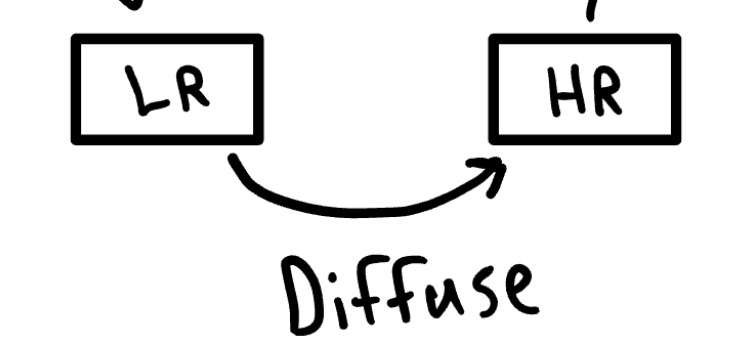
\includegraphics[width=\linewidth]{images/ls-diffuse.png}
    \end{column}
    % right column: bullets
    \begin{column}{0.48\textwidth}
      \begin{itemize}
        \item Trained diffusion layer yielded poor results for end-to-end segmentation run
        \item Things I've Tried:
        \begin{itemize}
          \item Deeper network (add conv & relu layers)
          \item W net (decode then encode again)
          \item Transformers
        \end{itemize}
      \end{itemize}
    \end{column}
  \end{columns}
\end{frame}

\begin{frame}{Pivot: Image to Image Diffusion Model}
    \centering
    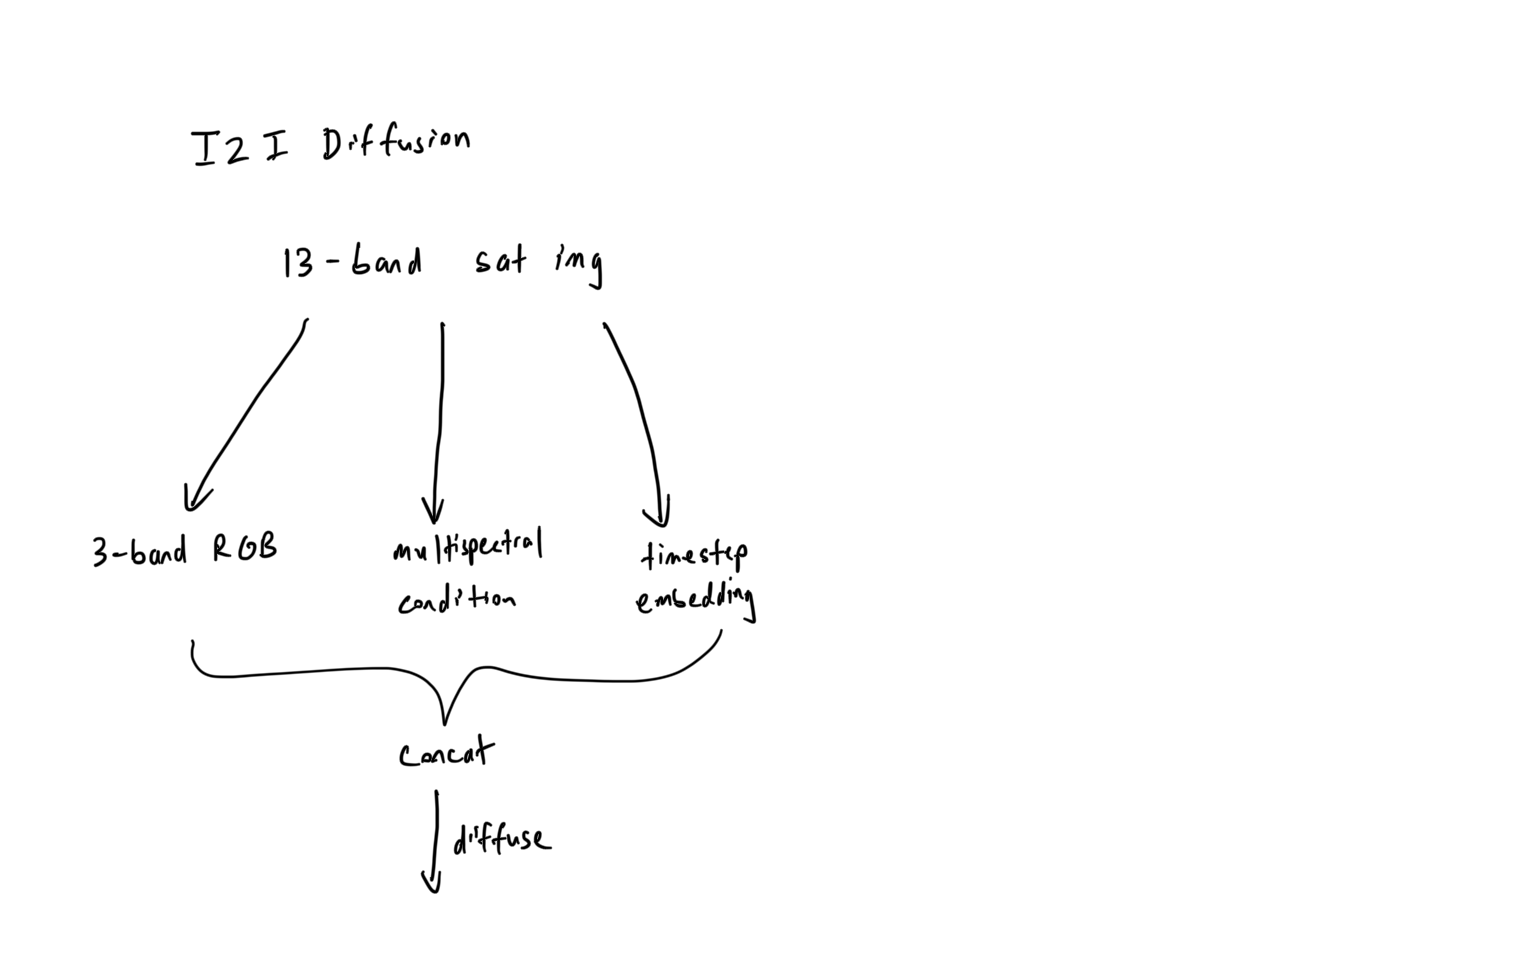
\includegraphics[height=0.7\textheight,width=0.7\textwidth,keepaspectratio]{i2i-diffuse.png}
\end{frame}

\begin{frame}{I2I Diffusion}
    \begin{enumerate}
        \item Runs on RGB bands of satellite image
        \item Diffusion conditioned on gated multispectral features and timestep embedding
        \item Completed train runner, train/eval steps, benchmark
    \end{enumerate}
\end{frame}
